\chapter{Diagnostic Models}
This section analyses distribution networks (also known as distribution systems). Distribution networks connect the nodes of a supply chain, that can have a worldwide extent. They involve the network infrastructure, i.e. roads, rails, water connections, air connection, pipelines and any other infrastructure needed to move goods from a point to another. Production network must be effective, by providing a fast and safe connection between customers and clients, and efficient since they add no value to the product transported.\par

Special attention must be paid in the design of the infrastructure of these networks.The capacity and the velocity of the connection make a country powerful and competitive in the international market.  The design and control of the distribution on the network is a crucial issue as well. Decisions as the type of vehicle, or the frequency of a connection heavily affect the efficiency of the network.\par

Distribution systems are modelled using the graph theory which is well explored from a mathematical and computational point of view; for this reason, there is room for the application of graph-based data-driven models in the field of distributions science.\par

This chapter focuses on the definition of the keywords and key entities extending the ontology of chapter \ref{chap_InformationFramework} to distribution systems. After that, it introduces the diagnostic framework for production nodes with a relational data structure. A non-relational data structure is introduced to overcome some limits of the relational data structure, enhancing data collection from multiple sources and more effective analysis to support the design and control of a distribution network.\par

Chapter \ref{chapDistControl} focuses on model-driven and data-driven approaches to control a distribution network. In contrast, chapter \ref{chapDistDesign} does the same to support the decisions on the design of a distribution network.

\section{Ontology} \label{secOntologyDistribution}
Here we go deeper into the details of the general ontology introduced in chapter \ref{chap_InformationFramework}. This chapter applies that approach to a distribution network that, in general, can be considered the biggest logistic system possible, since it is globally ditributed. 

\subsubsection{Entities}
We identify the following entities.\par
\textbf{Part} ($i$): A part is a handling unit (HU), i.e. the smallest part that is loaded and unloaded from a vehicle. The HU is usually the object of digital tracking in the supply chain. Depending on the type, and the extent of the network, a HU can be a carton (e.g. parcels supply chain), a pallet (e.g. supply chains with distribution centres), or even a container (e.g. globally distributed supply chain). \par

\textbf{Processing node} ($j$): The resources in charge of loading and unloading parts from vehicles. These entities are terminals, platform or bays, depending on the type of vehicle to load/unload (aircraft, vessels, trains, trucks, vans). \par

\textbf{Edge} ($j,k$):Any path connecting two processing nodes is an edge. Edges of a distribution network have a type, defining the type of vehicle able to travel on the edge (e.g. air, rail, water, road) and a capacity. \par

\textbf{Vehicle} ($v$): A vehicle is an element travelling on edges to transport HUs from a processing node to another. \par

\textbf{Consumable} ($s$): It models the energy or the fuel to operate vehicles. \par

\textbf{Route} ($e$): It is a predefined visiting sequence of different processing nodes. \par

\textbf{Order} ($o$): It is a transportation order received from a customer or generated by a freight forwarder. \par

\textbf{Job} ($b$): It is the schedule of the processing nodes to visit, including the expected service time windows and the detail of the HUs to load/unload. \par

\textbf{System network} The graph $G(V,A)$ of nodes $j\in V$ and edges $\left(j,k\right)\in A$ composing the distribution network.

\subsubsection{Metrics}
We identify the following metrics to assess the performances of a processing node $j$.\par

\textbf{Throughput} ($TH_{j}$): The productivity of a resource, i.e. the average number of HUs loaded and unloaded per unit of time (e.g., containers per hour).\par

\textbf{Work in process} ($WIP_{j}$): It is the number of parts stored in a location $j$.\par

\textbf{Work in process} ($WIP_{jk}$): It is the number HUs (i.e., the level of inventory) waiting to be loaded on a vehicle $v$. \par

\textbf{Capacity} ($C_j$): It is the upper bound of the throughput of a resource.\par

\textbf{Capacity} ($C_v$): It is the maximum number of HUs transportable by a vehicle $v$ at the same time. \par

\textbf{Utilisation} ($U_j$): It is the average fraction of time that a resource is not idle for lack of vehicles to load/unload. \par

\textbf{Utilisation} ($U_v$): It is the average fraction of non-empty space on a vehicle. \par

\textbf{Lead time} ($LT_e$): It is the time allocated to serve a given route (i.e. from the beginning to the end). \par

\textbf{Cycle time} ($CT_e$): It is the average time to serve a given route. \par

\textbf{Service level} ($SL_e$): $Prob\{cycle\ time\le lead\ time\}$

\subsubsection{Information functions}
Finally, we define the three information functions: Movements $M$ are referred to load/unload of HUs on vehicles $v$; inventories $I$ are referred to the work in process on a terminal $j$, or a vehicle $v$. The productivity $P$ refers to the inbound and outbound absorption rates of the terminal. Table \ref{tab_information_functions_dist} summarises the definition of the three functions in a distribution network.



% INSERT tab_information_functions_dist
\begin{figure}[hbt!]
\centering
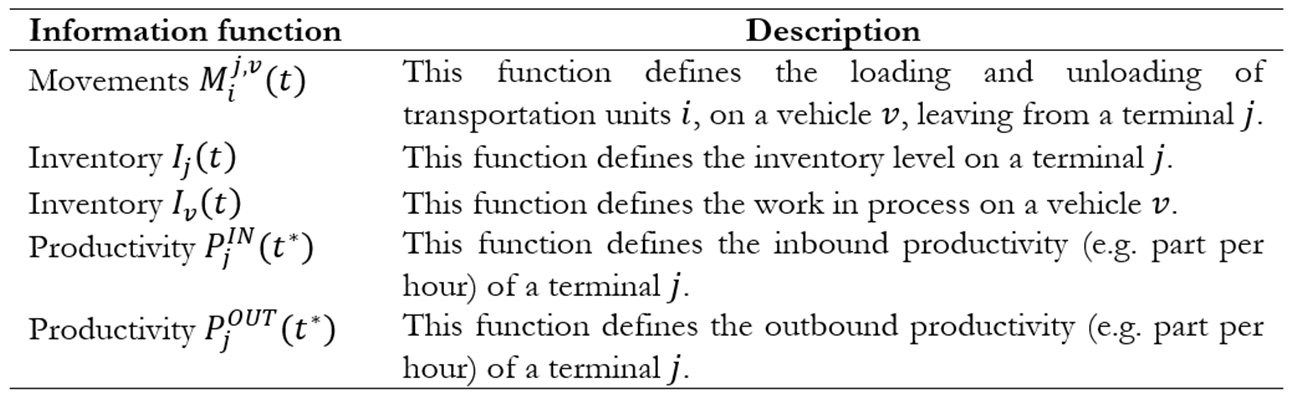
\includegraphics[width=1\textwidth]{SectionDistribution/diagnosticModels_figures/tab_information_functions_dist.png}
\captionsetup{type=table}
\caption{Definition of the information functions of a distribution network.}
\label{tab_information_functions_dist}
\end{figure}

\section{Data Structure}
In the supply chain field, data collection developed together with the concept of traceability. Robust relational data structures rose to control the shipping processes and identify the status of HUs. For this reason, all the data collected in a distribution network revolves around the shipping information. The bias of the data structure is shallow compared to other supply chain entities (e.g. production systems). HUs are similar, share similar vehicles, and they travel on a graph $G$ defined by nodes and edges where often the arcs refer to a finite and well-known set of elements (roads, rail tracks, air tracks or waterways). We present a relational data structure to study many aspects of a distribution network from a research point of view, keeping in mind that the ER structure is the most widely used in the shipping companies. Together with that, an original non-relational structure is introduced to overcome the rigidity of the relational structure and to improve the level of information from different players on the supply chain.

\subsection{A relational model for distribution networks} \label{secRelationalModelDist}

Organisational and industrial practice choose the entity-relationship (ER) model as the most used method to store and organise data. The outcome of this organisation is the well-known table structure of a SQL database. ER models use tables to describe the attributes of entities and define relationships to link entities that share the same attributes. Entities can be a part $i$, a vehicle $v$ or resource $j$ connected by relationships which describing a route $e$, or a job $b$. A SQL database provides many benefits in a production environment as:
\begin{itemize}
    \item Low replication of data since tables are structured in the so-called normal form;
    \item Easy access to data. The SQL language allows programmers to get data just thinking of which data do they need and not how to fetch that data from the database;
    \item High data consistency; since relationships impose relational integrity which prevents from adding sparse data.
\end{itemize}

The ER model we propose is organised into three macro-areas of a distribution network aiming at providing a comprehensive framework to model a distribution network ~\cite{Accorsi2018}:

\begin{enumerate}
    \item A geographical level;
    \item A logistic level;
    \item An on-field level.
\end{enumerate}

The entities and relationships belong to each of these areas.
\subsubsection{Geographical level}

The geographical level aims at defining the characteristic of macro-areas of the world called \textit{Geoareas} from a geopolitical perspective. A table \textit{SocioEconomicProfile} identifies the statistics on the GDP, inflation and other similar indicators. The table \textit{AgroProfile} tracks the characteristics of the soil while the table \textit{ClimateProfile} tracks the weather and climate trends. The table \textit{InfrastructureProfile} maps the transport infrastructure of a \textit{Geoarea} while the table \textit{LogisticProfile} contains aggregated logistics indicators as the import and export volumes. The tables \textit{InfrastructureCostProfile} and \textit{EnergyCostProfile} identify the average costs of the infrastructures (e.g. buildings, land, licences) and the price for consumables (e.g. electricity). A table \textit{DemandGeoArea} has aggregated values of demand for clusters of similar products (e.g. fruits, vegetables, potatoes) within the \textit{Geoarea}. Table \ref{tab_geo_attributes} illustrates the details of the attributes for each table of the geographical level.


% INSERT tab_geo_attributes
\begin{figure}[hbt!]
\centering
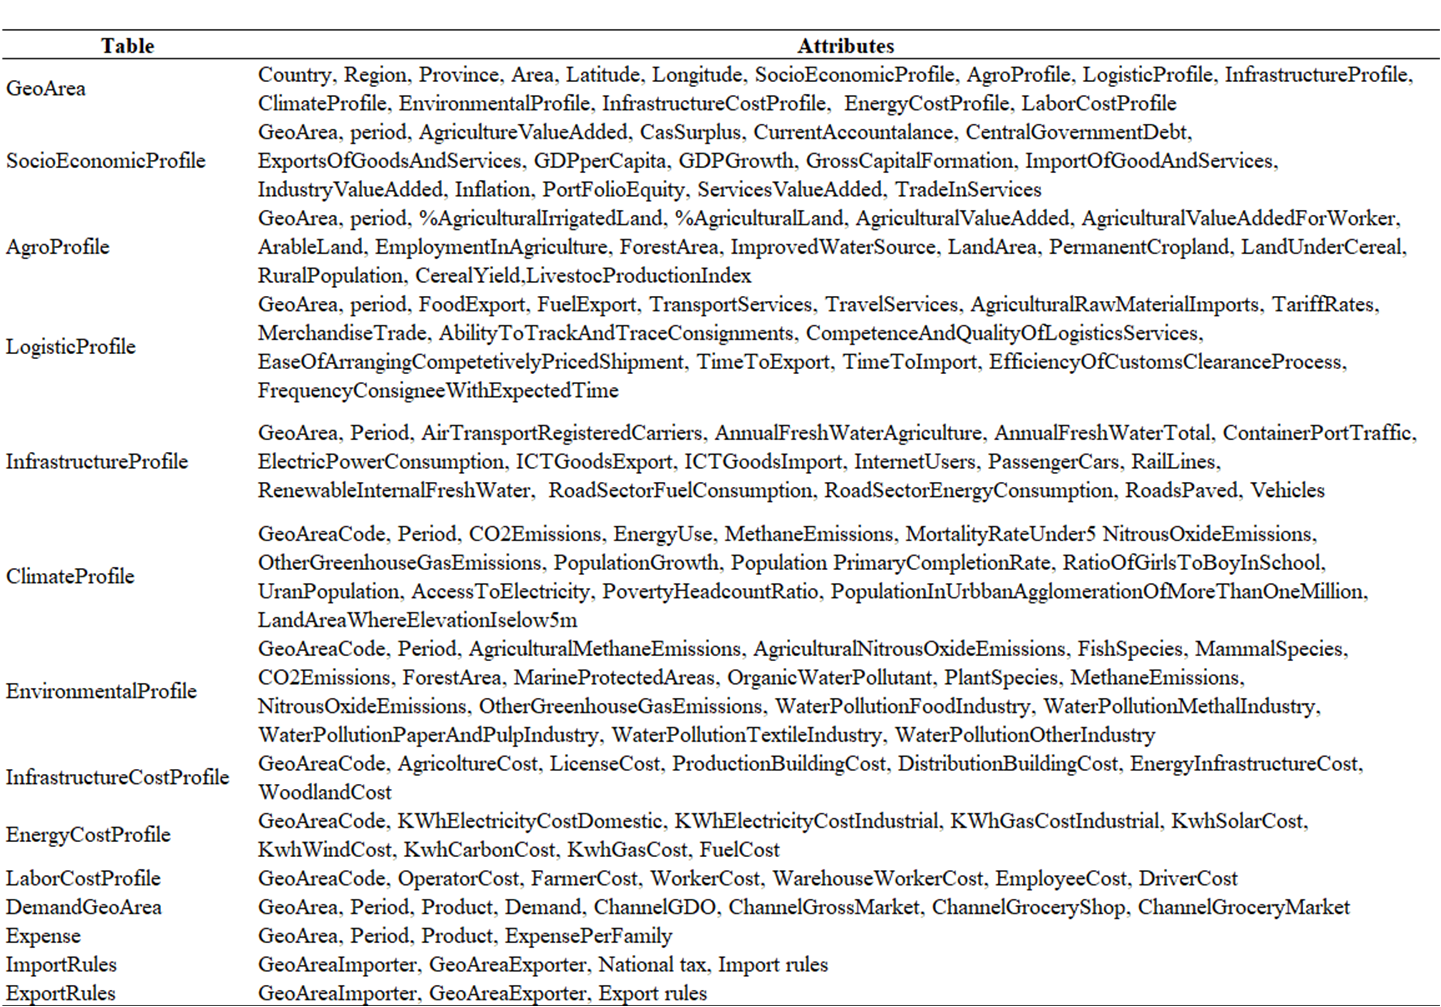
\includegraphics[width=0.9\textwidth]{SectionDistribution/diagnosticModels_figures/tab_geo_attributes.png}
\captionsetup{type=table}
\caption{Tables and attributes of the geographical level.}
\label{tab_geo_attributes}
\end{figure}


\subsubsection{Logistic level}

The logistic level contains all the entities to populate the ontology presented in \ref{secOntologyDistribution}. A table node identifies all the processing nodes of the network connected by the edges whose material flow is mapped in the table \textit{Flow}. Each row of the table \textit{Node} identifies s a processing node of a specific type. Depending on the node type, the tables \textit{Crop}, \textit{ProcessingPlant}, \textit{StorageFacility}, \textit{Market}, \textit{Port}, \textit{Terminal}, \textit{MultimodalHub}, and \textit{RailConnection} identify the characteristics of the node. Table \ref{tab_log_attributes} illustrates the details of the attributes for each table of the logistic level.


% INSERT tab_log_attributes
\begin{figure}[hbt!]
\centering
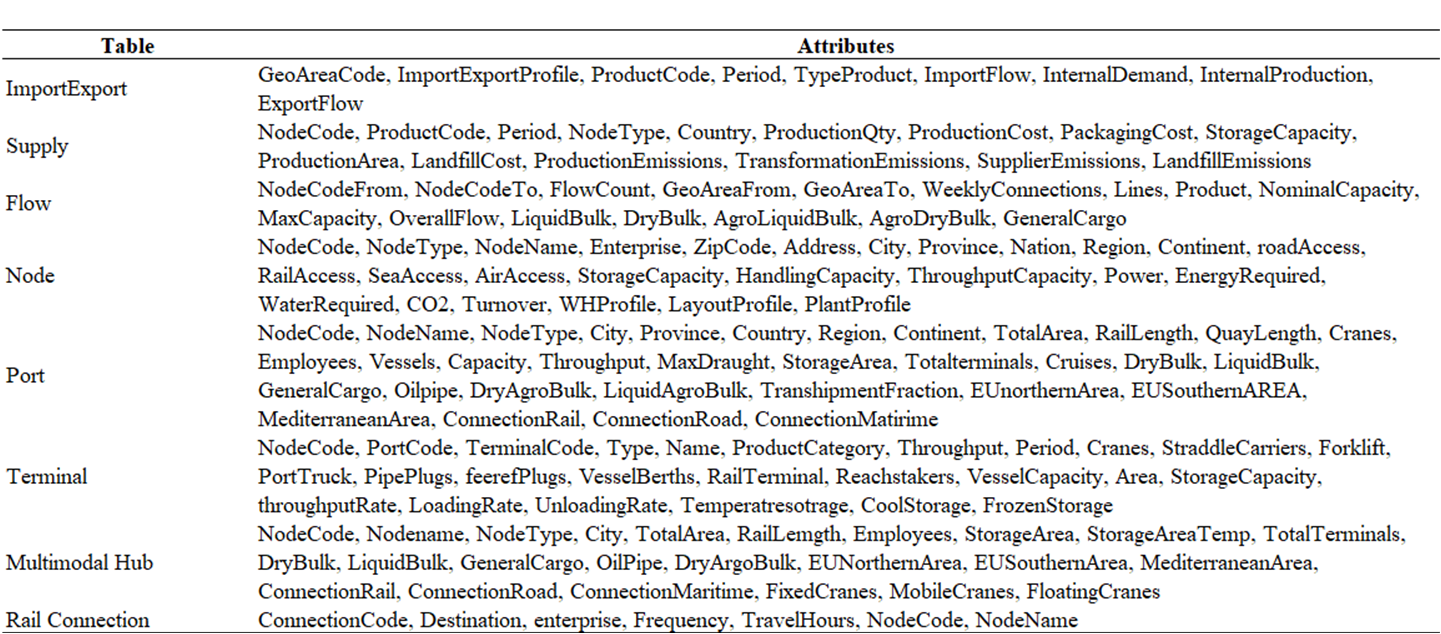
\includegraphics[width=0.9\textwidth]{SectionDistribution/diagnosticModels_figures/tab_log_attributes.png}
\captionsetup{type=table}
\caption{Tables and attributes of the logistic level.}
\label{tab_log_attributes}
\end{figure}


\subsubsection{On-field level}

The on-field level deals with the track\&trace world collecting the shipping logs and all the related information. The table order contains all the shipping orders (i.e. provisional data) from a processing node $j$ to a processing node $k$. The table shipment contains all the shipping jobs (i.e. execution data) of the shipping orders from $j$ to $k$. The table product map is the item master file containing all the details (e.g. code, size, volume, weight) of the items. A product mapped in this table is equal to the definition of a part in a production node (see section \ref{secDataStructureProduction}). A table shelflife identifies the quality decay rates of each item. The tables package and unitLoad maps all the features of the handling units (HU). A table \textit{ClimateProfileMonitoring} contains the temperature logs of shipping. Table \ref{tab_onfield_attributes} illustrates the details of the attributes for each table of the on-field level.

% INSERT tab_onfield_attributes
\begin{figure}[hbt!]
\centering
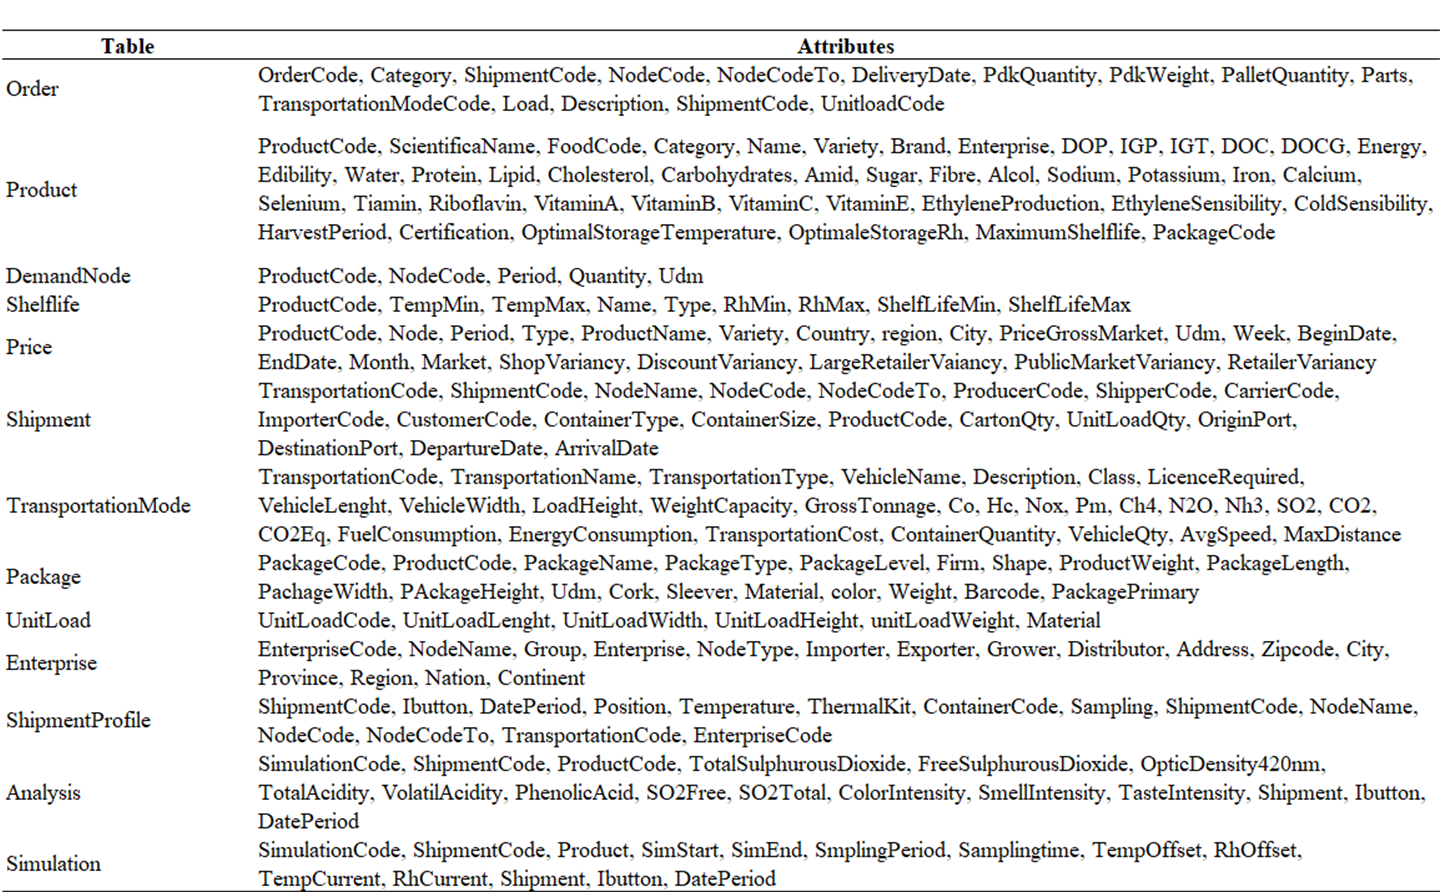
\includegraphics[width=0.9\textwidth]{SectionDistribution/diagnosticModels_figures/tab_onfield_attributes.png}
\captionsetup{type=table}
\caption{Tables and attributes of the on-field level.}
\label{tab_onfield_attributes}
\end{figure}

Figure \ref{fig_dist_ER_model} presents the resulting ER structure with the tables belonging to the three levels.

% INSERT fig_dist_ER_model
\begin{figure}[hbt!]
\centering
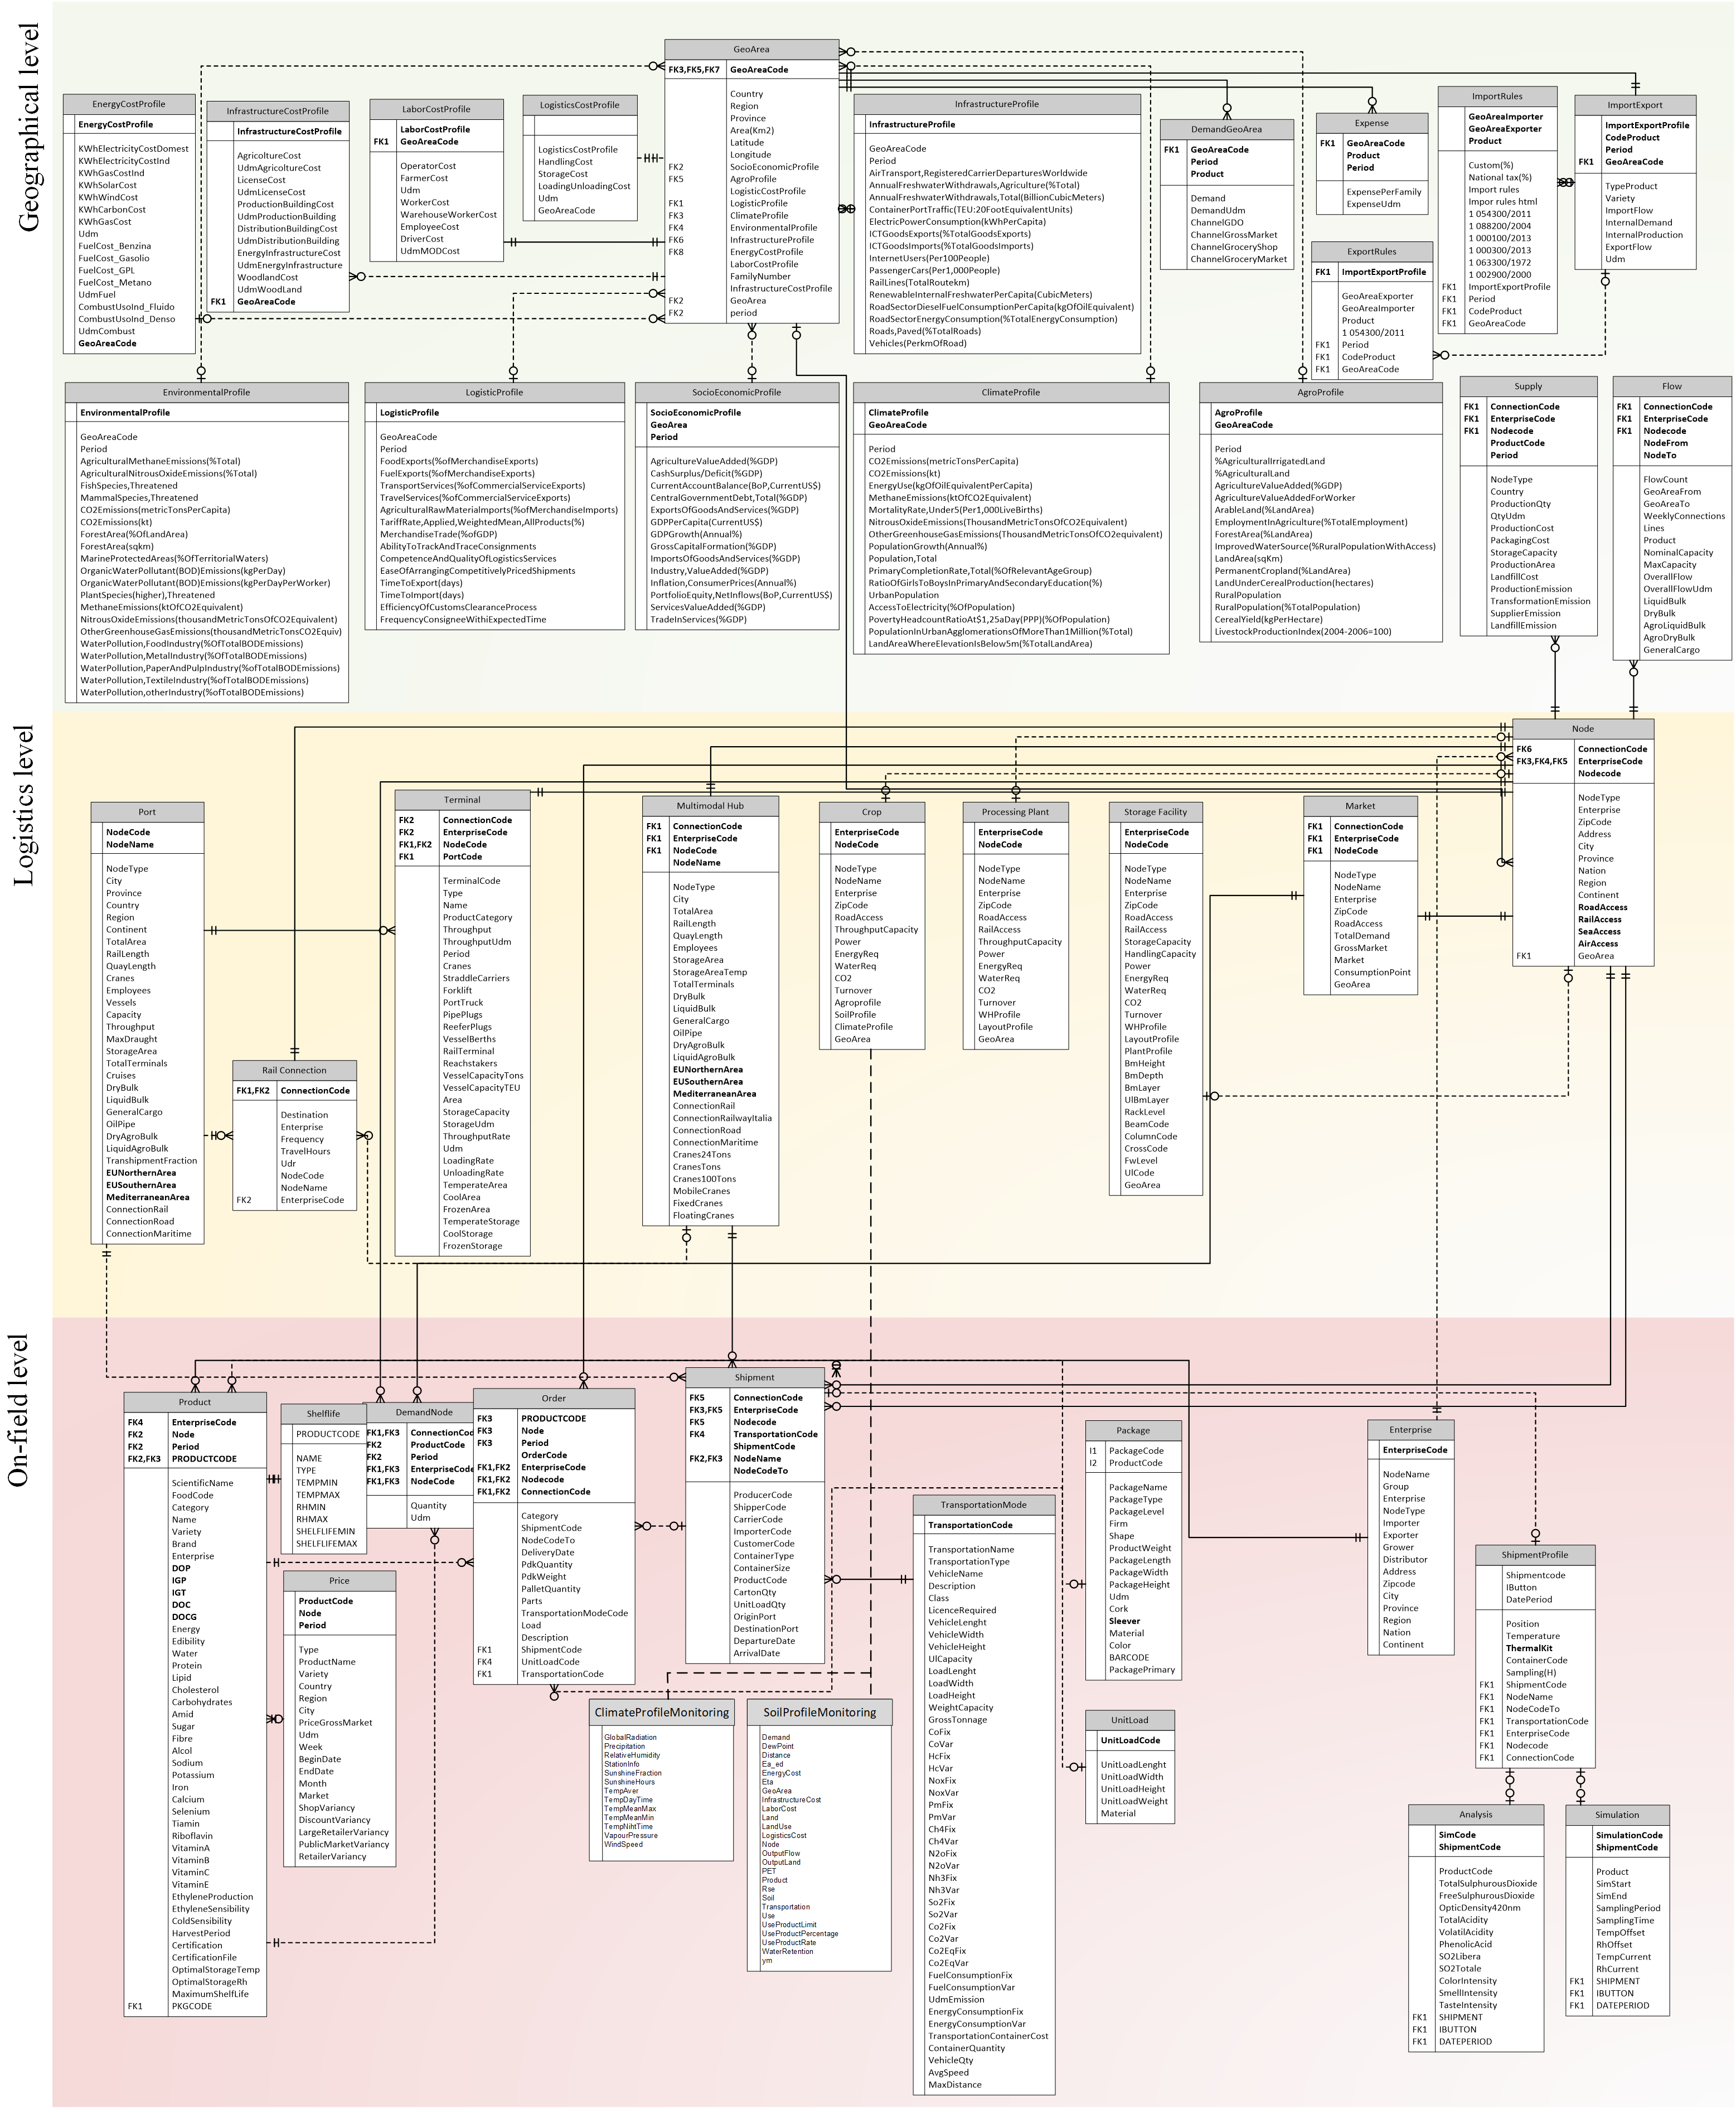
\includegraphics[width=0.9\textwidth]{SectionDistribution/diagnosticModels_figures/fig_dist_ER_model.png}
\captionsetup{type=figure}
\caption{ER diagram of the relational data struvture for distribution networks.}
\label{fig_dist_ER_model}
\end{figure}


\subsection{A non-relational model for distribution networks}
This section presents a non-relational data structure able to embed the same information content of the ER model introduced in \ref{secRelationalModelDist} but able to host any other additional attribute.  Besides, the model has a minimum number of required attributes that enables define a minimum viable model (MVM). The MVM contains a number of mandatory attributes for each class of the model allowing analysis of a supply chain network. The classes of the non-relational model are the natural implementation of the MIP model introduced in Section \ref{secInfoFramework}. \par

A non-relational data-structure is usually stored in a computer using a JSON or XML notation. Non-relational structures are widely used in web application with databases as MongoDB since they allow to store tons of data in an (apparently) unstructured way without the prior definition of any table or relationship. Each record of the database is a \textit{document} of a \textit{collection}. These characteristics lead to many benefits as:

\begin{itemize}
    \item the high flexibility of the data structure, since it is possible to load data with or without attribute already stored in a collection;
    \item the fast data fetching due to a leaner structure compared to SQL databases;
    \item the scalability of the data structure since the performance of the database is not directly related to its size.

\end{itemize}

These benefits come with some important limitations:

\begin{itemize}
    \item many data may be replicated, leading to data storage inefficiencies. Due to the lack of relationships, information can be replicated in many documents with inefficiencies in the use of the storage space;
    \item join operations are not allowed. When a join operation is needed, it is necessary to perform it externally and without query optimisation;
    \item data are not as consistent as with an ER model; Since relations does not exist, it is impossible to store consistent data. Data consistency check must be performed outside of the database.

\end{itemize}

The model consists of three collections whose data are recorded by the transportation management system (TMS). \par

A collection \textit{handling units} identifies all the parts i transported on the network. The code of the handling unit is the only attribute necessary to define the MVM. Other attributes can be stored as well, like:

\begin{itemize}
    \item the description
	\item the size, 
    \item the weight,
    \item the dimension,
    \item the type of package (e.g. primary, secondary, tertiary).
\end{itemize}

A collection \textit{movement} defines the movement function of the MIP model, storing information on when a part $i$ is loaded or discharged by a vehicle $v$. The timestamp and the quantity are the attributes needed for the definition of the MVM. Other features can be recorded, as for example:

\begin{itemize}
    \item the id of the loading node, 
    \item the id of the discharging node,
    \item the latitude and longitude of the loading node,
    \item the latitude and longitude of the discharging node,
    \item the provisional loading time window,
    \item the actual loading time window,
    \item the provisional discharging time window,
    \item the actual discharging time window,
    \item the id of the vehicle,
    \item the id of the voyage.
\end{itemize}

A collection \textit{node} stored the information of all the suppliers and customers of the supply chain network. The id of the node is enough to define the MVM. It is possible to record a attributes as:

\begin{itemize}
    \item the description,
    \item the latitude and longitude of a node,
    \item the address of a node, 
    \item the type of the node (i.e. supplier/customer),
    \item the list of the material flows exchanges every year with a given node (e.g. the production plant serving the distribution network).
\end{itemize}

This non-relational structure is used in the rest of this section to support model and analysis on production systems. Figure \ref{fig_MVM_dist} uses the unified modelling language (UML) to represent the MVM of the non-relational data structure of a distribution network.

% INSERT fig_MVM_dist
\begin{figure}[hbt!]
\centering
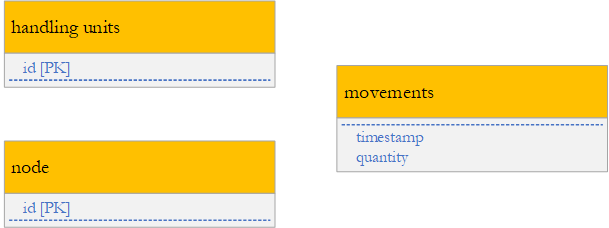
\includegraphics[width=0.9\textwidth]{SectionDistribution/diagnosticModels_figures/fig_MVM_dist.png}
\captionsetup{type=figure}
\caption{ER diagram of the relational data structure for distribution networks.}
\label{fig_MVM_dist}
\end{figure}


\section{Decision patterns} \label{secDecisionPatternsDistribution}
This section aims at defining the set of decision patterns for the design and control of a distribution system, according to the definitions of section \ref{secDecisionPatterns}. The problems of a distribution system are classified into:

\begin{enumerate}
    \item Network design problems, dealing with the design of the network, given the existent physical infrastructure;
    \item Network control problems, dealing with the assessment and improvement of the performance of an existing distribution network.
\end{enumerate}

Different methodologies allow getting feasible solutions to these problems. Table \ref{tab_problems_dist} illustrates the entities and their definition according to the ontology in Paragraph \ref{secOntology}. 

% INSERT tab_problems_dist
\begin{landscape}
\thispagestyle{empty}
\begin{figure}[hbt!]
\centering
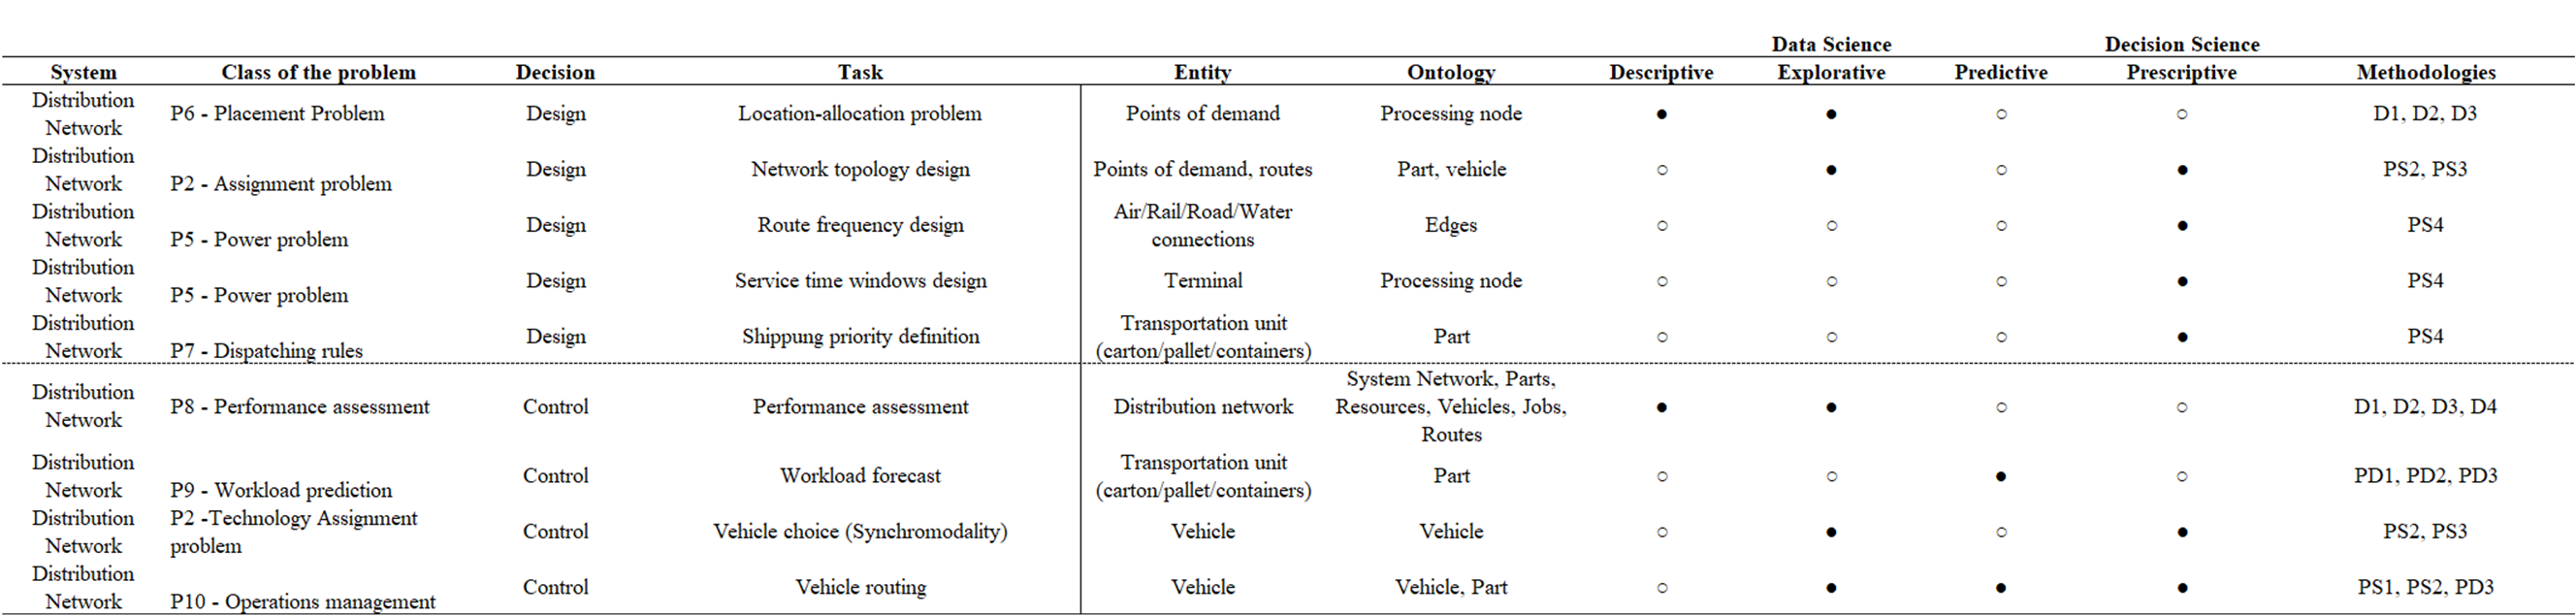
\includegraphics[width=1.5\textwidth]{SectionDistribution/diagnosticModels_figures/tab_problems_dist.png}
\captionsetup{type=table}
\caption{Decision problems classification in a distribution system.}
\label{tab_problems_dist}
\end{figure}
\end{landscape}

Seven decision problems are identified in the design and control of a storage node:

\begin{enumerate}
    \item Network design; it is a covering problem where each point node of the network needs at least one route serving it.
	\item Route frequency design; it involved the definition of the frequency of the service on a given route.
	\item Service time windows design; it is the definition of the placement and the time span of the time windows to serve each node $j$.
	\item Performance assessment (control); it involves the measurement of the performance of a distribution system.
	\item Workload forecast (control); it involves the prediction of the workload and workforce needed to perform the operation in the short-, mid- or long-term.
	\item Vehicle choice; it is the choice of the right vehicle (or the right type of vehicle in case of synchromodality) to perform a route.
	\item Vehicle routing (control); it involves the definition of the scheduled routes and their assignment to vehicles.

\end{enumerate}

While descriptive and prescriptive techniques are preferred for control problems, explorative and prescriptive techniques result adequate when dealing with design problems. Chapters \ref{chapDistControl} and \ref{chapDistDesign} illustrate these techniques in details.






%\clearpage
\bibliographystyle{ieeetr}
\bibliography{SectionDistribution/diagnosticModels_ref}